\documentclass[11pt,letterpaper]{article}

\usepackage[english]{babel}
\usepackage[utf8]{inputenc}

\usepackage{amsmath}
\usepackage{amssymb}
\usepackage{graphicx}

\usepackage[top=1in, bottom=1in, left=1in, right=1in]{geometry}
\graphicspath{{./imagenes/}}

\begin{document}
	
	\begin{titlepage}
		\centering
		
		{\scshape\LARGE Universidad Nacional Autónoma de México \par}
		
		\vspace{1cm}
		{\scshape\Large Facultad de Ciencias\par}
		\vspace{1.5cm}
		
		\begin{figure}[h]
			\centering
			
\includegraphics[scale=0.15]{logo.png}
		\end{figure}
		
		\vspace{.8 cm}
		
		{\LARGE Práctica 02 \par}
		
		\vspace{0.5cm}
		\large{\itshape{Vianey Aileen Borrás Pablo}} \small{ - 316033619} \\ \vspace{0.3cm}
		\large{\itshape{Kevin Axel Prestegui Ramos}} \small{ - 316201373} \\ \vspace{0.3cm}
		\vfill
		
		\textbf{Arquitectura de Computadoras}\\
		\textbf{Dr. Jorge Luis Ortega Arjona}. \par
		\vspace{0.5cm}
		Fecha de entrega: \textbf{12 de marzo de 2020}.
	\end{titlepage}

	
	\begin{itemize}
		\item \textbf{Pregunta 1}\\
		
		Reduce con mapas de Karnaugh la siguiente representación de circuito.\\
		
		WXYZ + WXY$\overset{-}{Z}$ + WX$\overset{-}{Y}$$\overset{-}{Z}$ + W$\overset{-}{X}$$\overset{-}{Y}$Z + $\overset{-}{W}$$\overset{-}{X}$ $\overset{-}{Y}$Z + WX$\overset{-}{Y}$Z
		
		\begin{figure}[h]
			\centering
			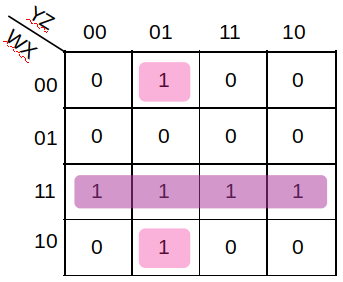
\includegraphics[scale=0.5]{MapaKarnaugh.png}
			\caption{Mapa de Karnaugh}
		\end{figure}
	
		Entonces la fórmula minimizada es: WX + $\overset{-}{X}$$\overset{-}{Y}$Z
		
		\item \textbf{Pregunta 2}\\
		
		Considerando el siguiente enunciado:\\
		
		\textit{El club de Tobi tiene 3 integrantes aparte de Tobi, como este no está, a los 3 integrantes se les ocurre realizar un motín para cambiar el nombre del club. Puesto que el club es de Tobi, él es el único que su voto vale doble.} 
		
		\subitem \textbf{- Tabla de verdad que indica si se realiza el motín.}\\
			\hspace*{0.85cm} Recordemos que Tobi no está por lo que la tabla de verdad será de tres variables.
			
			\begin{figure}[h]
				\centering
				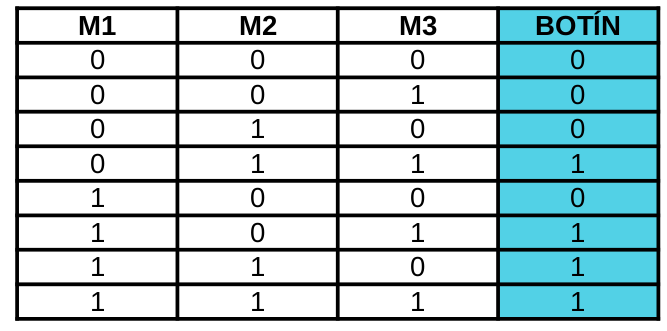
\includegraphics[scale=0.45]{Motin.png}
				\caption{Tabla de verdad: Motín}
			\end{figure}
		
		\newpage
		\subitem \textbf{- Función booleana}\\		
		\hspace*{0.85cm} Con base a la tabla de verdad se obtiene la siguiente función booleana.
		
		\hspace*{3.5cm} $\overset{-}{M_{1}}M_{2}M_{3} + M_{1}\overset{-}{M_{2}}M_{3} + M_{1}M_{2}\overset{-}{M_{3}} + M_{1}M_{2}M_{3}$
		
		\subitem \textbf{-Reducción de la función booleana}\\
		\hspace*{0.85cm}Reduciendo con mapas de Karnaugh tenemos:
		
		\begin{figure}[h]
			\centering
			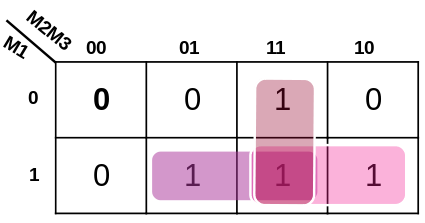
\includegraphics[scale=0.5]{Karnaugh.png}
			\caption{Mapa de Karnaugh del motín}
		\end{figure}
	
		\hspace*{0.85cm} Entonces la fórmula reducida es:\\
		\hspace*{0.85cm} \textbf{Motín} = $M_{1}M_{3} + M_{2}M_{3} + M_{1}M_{2}$
		
		
		\item \textbf{Pregunta 3}\\
		
		El siguiente circuito puede ser representado por una sola compuerta,\\
		¿Cuál? Justifica.
		
		\begin{figure}[h]
			\centering
			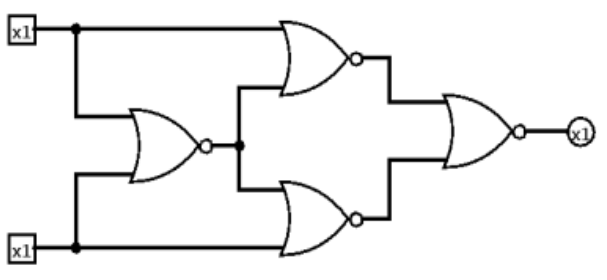
\includegraphics[scale=0.40]{Pregunta3.png}
		\end{figure}
	
		Observemos que nuestra función resultante de dicho circuito es $\overline{\overline{(X+\overline{(X+Y)})}+\overline{(Y+\overline{(X+Y)})}}$, representando dicha función en tabla de verdad podemos darnos cuenta que es equivalente a si usaríamos la puerta XNOR.
		
		\begin{figure}[h]
			\centering
			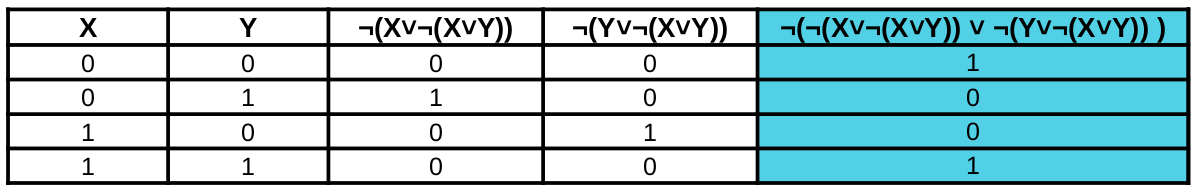
\includegraphics[scale=0.35]{EquivXNOR.png}
			\caption{Tabla de verdad del circuito}
			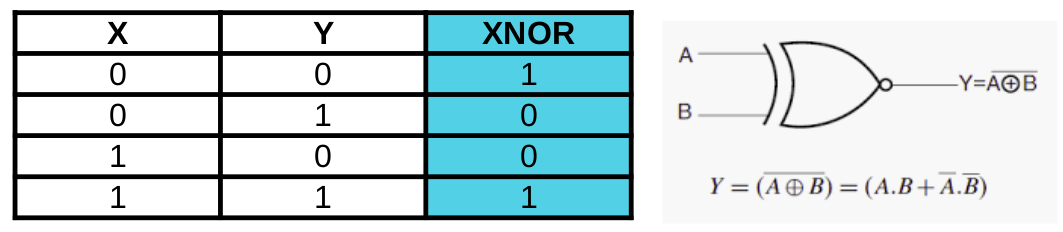
\includegraphics[scale=0.35]{XNOR.png}
			\caption{Tabla de verdad XNOR}
		\end{figure}
		
		\newpage
		\item \textbf{Pregunta 4}\\
		Determina la expresión correspondiente para el siguiente circuito. Justifica.
		
		\begin{figure}[h]
			\centering
			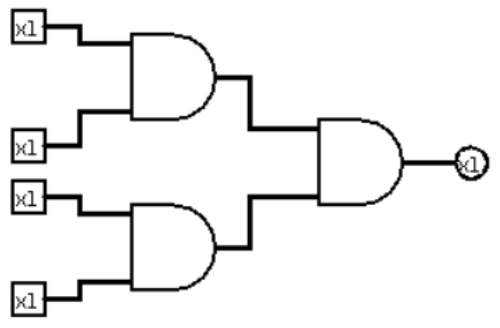
\includegraphics[scale=0.30]{Pregunta4.png}			
		\end{figure}
	
	Observemos que el circuito esta formado por tres puertas AND por lo que la expresión correspondiente es ABCD.
	
	\begin{figure}[h]
		\centering
		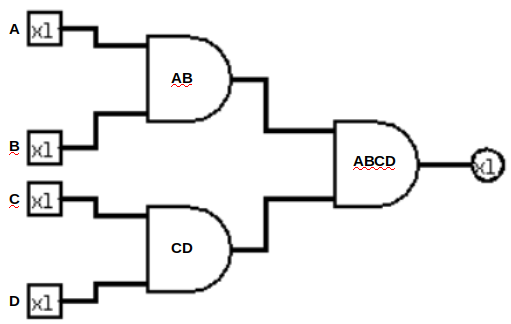
\includegraphics[scale=0.35]{CircExpr.png}
		\caption{Justificación de la expresión}
	\end{figure}
		
	\end{itemize}		

\end{document}